\chapter{Sample File}
In this \textbf{sample file} we discuss how easy it is to use latexToHtml.

First, some headlines:

\section{Section}
\subsection{Subsection}
\subsubsection{Subsubsection}
\subsubsection{Paragraph}
\paragraph{Paragraph}
\subparagraph{Subparagraph}

\label{sec:equation}
\section{Equations} 

Equations can be written line such as $x = 3 + 5$, or you can use the equation environment as shown in Equation~\ref{eqn:sample}.

\begin{equation}
\label{eqn:sample}
\frac{1+sin(x)}{y}
\end{equation}

\thiswontshow

\section{Footnotes}  
Footnotes\footnote{Footnotes are information about the annotated word/phrase} will be underlined and the information shows when hovering over them\footnote{You can also put URLs such as \url{http://palladian.ws} in footnotes}.

\section{Images}
Images, such as Figure \ref{fig:sample} can be added too. Figure \ref{fig:samplePng} shows a png file. 

\begin{figure}
\centering

\includegraphics[width=4in]{pngFigure.png}
\caption{Sample PNG Figure}
\label{fig:samplePng}
\end{figure}

Figure \ref{fig:samplePdf} shows an embedded pdf file.
 
\begin{figure}
\centering
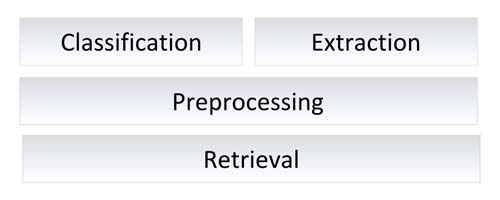
\includegraphics[width=4in]{pdfFigure.pdf}
\caption{Sample PNG Figure}
\label{fig:samplePdf}
\end{figure}